\section{Results}
\label{sec:results}

An important aspect of our methods is that deconvolution is not the same as a
shift. \attn{We need a concise description of this somewhere, possibly with a
graphic.}


\subsection{Infection estimates reveal waves missed by reported cases}
\label{sec:omitted-waves}

Outbreaks in infections precede those in reported cases and are reliably larger
in magnitude. But simply shifting cases back in time and increasing them by some
factor fails to capture the spatio-temporal dynamics of the pandemic. 
Hence, relative to reported cases, examining estimated infections reveals a
rather different pattern. \autoref{fig:state_infect_est} shows
estimates of the number of daily new infections per 100,000 inhabitants for each
\US state from June 1, 2020 to November 29, 2021 compared with reported cases,
and deconvolved cases (reported cases ``pushed back'' by the delays shown in
\autoref{fig:chain_events_onset_report}). 

While the major Ancestral, Alpha, and Delta waves tend to be visible for most
states, there are clear outbreaks in unreported infections that are not easily
detectable from cases alone in the falls of 2020 and 2021. For example, a wave 
of infections is present in the spring of 2021 for North Dakota and South Dakota
which is not visible in reported cases alone. \attn{we should search for more of
these patterns.}

\subsection{Spatial-temporal implications are ignored}
\label{sec:ignored-patterns}

\attn{We need to expand the discussion of this figure along the lines we
discussed in our meeting. Choose the dates carefully to emphasize that the
spatial extent during peaks/troughs of waves is different if you look at
infections instead of cases.}

\autoref{fig:choro_inf_case_rates} shows that for the
earliest time of June 1, 2020, there is little discrepancy between case and
infection rates, while for the later times there are immense differences in the
rates, such that case rates tend to underrepresent infections to a great extent.



\subsection{Infection/case ratios vary by state and VOC}
\label{sec:case-infection-ratio}

\attn{The rest of this section uses a lot of space to say, basically, that
infections are bigger than cases. I think we should cut much of it (though see
also below). I think a
better use is to more explicitly emphasize how the case/infection ratio changes
with time and VOC. Let's make that more focused, direct. Note that this isn't
really ``underreporting'', they're still reporting all the tests, but those
tests capture different numbers of infections.}

With respect to variants of concern, consider the late 2020
Ancestral wave for the midwestern states of Illinois, Indiana, and Ohio. For the
major Delta wave, some of the greatest discrepancies between cases and
infections are visible in the western states of Idaho and Montana, the southern
states of Louisiana and Georgia, and the midwestern states of Iowa and Nebraska
(\autoref{fig:state_infect_est}). Earlier on in the pandemic, such discrepancies
between cases and infections may be more attributable to failures in the
reporting pipeline, while later on in the pandemic, they more likely due to the
rise in asymptomatic infections across variants \citep{oph2022covid,
garrett2022high}. 

Finally, while the main Delta wave is somewhat evident from the case counts for
all states (\autoref{fig:state_infect_est}), our estimates suggest that case
counts tend to severely underestimate infections during this time for many
states. The lowest of all states was in New Jersey, where about $4.6\%$ (95\%
confidence interval: $[1.9, 67.7]$) of the estimated infections were reported.
This was followed by Maryland with $7.4\%$ ($[2.7, 83.8]$), Connecticut with
$8.0\%$ ($[3.1, 25.8]$), and Florida with $8.7\%$ ($[4.8, 34.0]$). This
underreporting issue extends to most states as in $39$ states less than $30\%$
of infections were reported during this time. Only $4$ states of Alaska, Maine,
Vermont and Virginia reported at least $40\%$ infections. No states were found
to surpass $50\%$ for reported infections for this time.

Similar patterns were observed during the earlier period of Alpha domination,
where Louisiana had the lowest reported infections at $11.7\%$ (95\% confidence
interval: $[6.7, 31.5]$) and was followed by California at $14.4\%$ (95\%
confidence interval: $[7.7, 68.2]$). There were $23$ states that reported at
least $40\%$ and $22$ states that reported at least $50\%$ of their infections.

Such patterns were comparatively less apparent during the earlier and larger
period of Ancestral domination, where Ohio and Maryland held the lowest
percentages of reported infections at $22.0\%$ (95\% confidence interval:
$[16.2, 34.0]$) and $22.3\%$ (95\% confidence interval: $[14.8, 40.5]$),
respectively. During this time, $28$ states that reported at least $40\%$ and
$14$ states that reported at least $50\%$ of their infections. 

\begin{figure}[!tb]
    \centering
        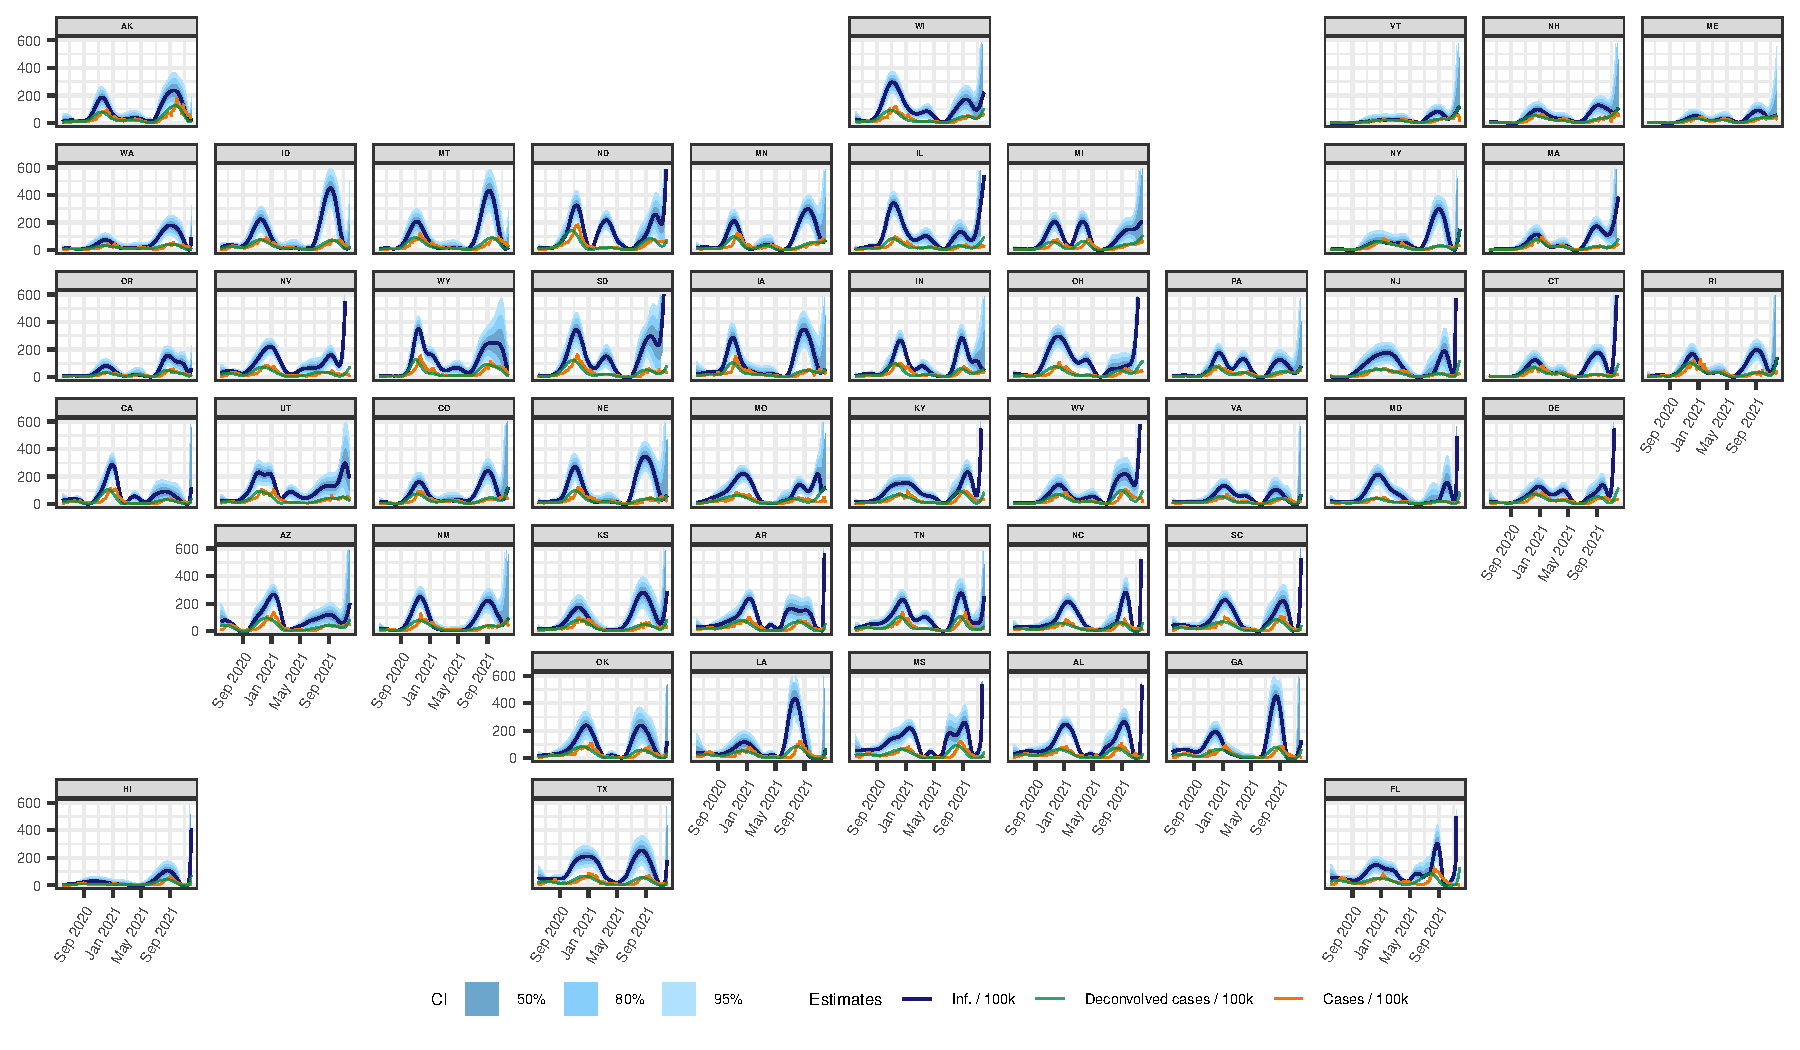
\includegraphics[width=.99\linewidth]{state_niauc_est_faceted_F24.pdf} 
        \caption{Estimates of the number of daily new infections per 100,000
            population for each \US state from June 1, 2020 to November 29, 2021
            (dark blue line). The blue shaded regions depict the 50, 80, and 95\%
            confidence intervals for the estimates, while the teal line represents
            the number of new daily new deconvolved cases per 100,000, and the
            dotted orange line represents the 7-day average of the new cases per
            100,000 as of the same date.}
        \label{fig:state_infect_est}
    \end{figure}
    

\begin{figure}[!tb]
\centering
    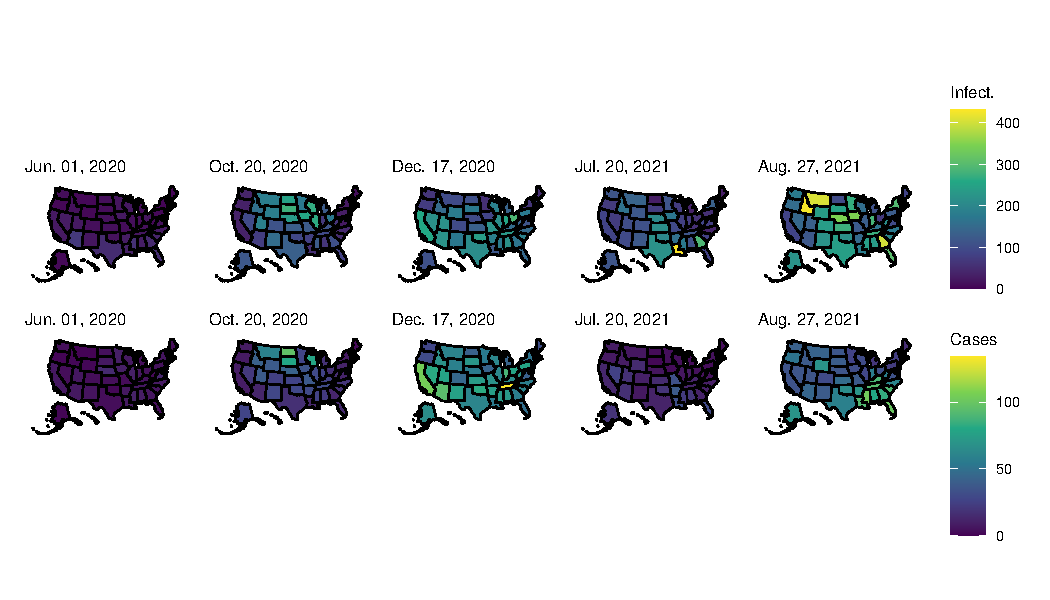
\includegraphics[width=.99\textwidth]{choro_inf_case_rates_F24.pdf}
    \caption{Choropleth maps of the state-level estimates of the number of daily
    new infections per $100,000$ population (top row) and the daily new cases
    per $100,000$ population (bottom row) for three times over the June 1, 2020
    to November 29, 2021 period. The first date was chosen simply as a baseline,
    while the second and third dates were chosen based on the day that had the
    largest number of infections across the 50 states from each year.} 
    \label{fig:choro_inf_case_rates}
\end{figure}    



    
\subsection{Infections broken down by VOCs emphasize earlier outbreaks}
\label{sec:infections-by-voc}

\autoref{fig:six-states} examines the infection estimates for a selection of
states more closely. This set has the largest infection/case ratios. 
\attn{We need to say more about what these 2 figures show, uniquely. What's the
point of looking at them? I think the section heading I wrote is the point. But
we need to say this. The takeaways below are a bit too vague, I think.} The top
panel shows \attn{....} The bottom panel divides estimated
infections into buckets based on the circulating variant proportions at the
time. From these plots, it is clear that few variant categories tends to
dominate and drive infections at a time. The general progression in terms of
variant starts with the Ancestral category from 2020 up to early 2021, to the
Alpha variant in mid 2021, which eventually gets eclipsed by the Delta variant
in mid to late 2021. This supports our division of our results by the three main
variant-driven time periods.


\begin{figure}[!tb]
\centering
    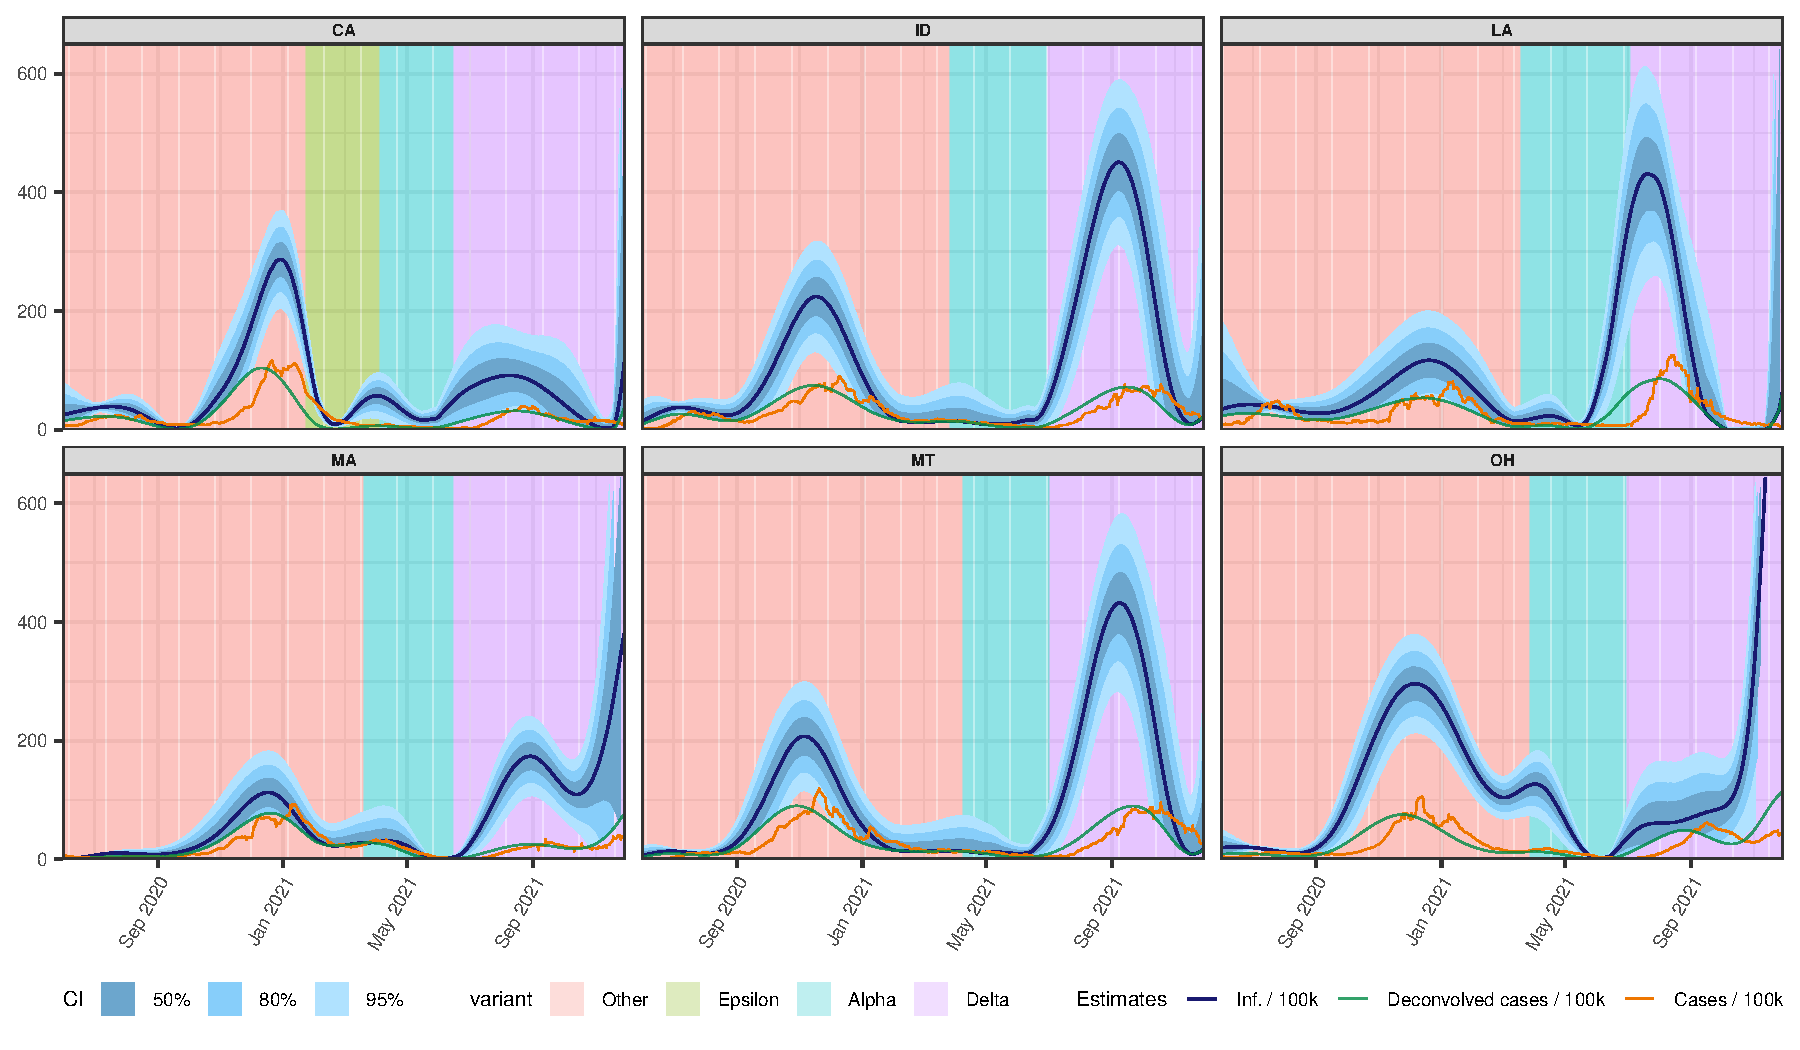
\includegraphics[width=\linewidth]{state_niauc_est_6states_F24.pdf}\\
    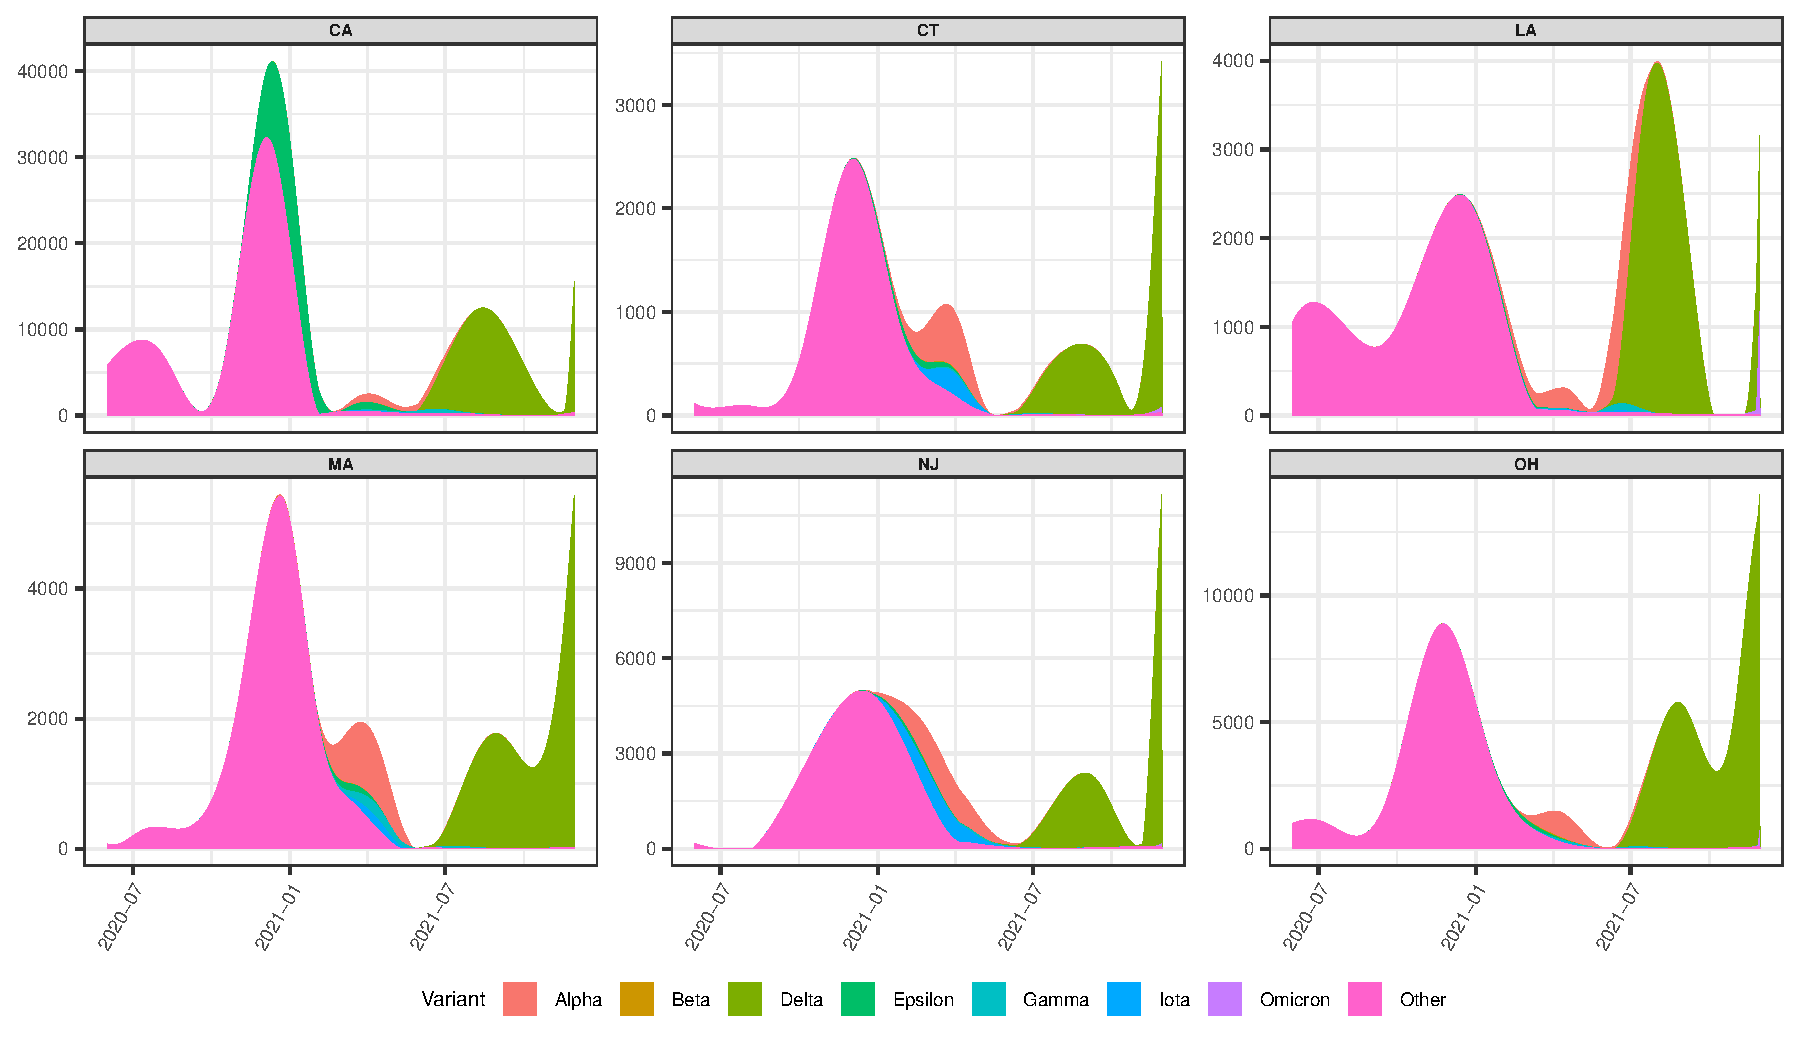
\includegraphics[width=\linewidth]{state_decon_byvar_est_6states_F24.pdf}
    \caption{Top panel: Reported cases, deconvolved cases, and estimates of daily new infections (dark blue
    line) per 100K inhabitants. The blue shaded regions indicate the 50, 80, and 95\% confidence
    bands, while the background is shaded to indicate the dominant variant in
    circulation at the time. \attn{I don't like the rotated x-axis.} 
    Bottom panel: Deconvolved cases colored by variant per 100K inhabitants. \attn{Is
    this the correct units? or are these raw? They should be per 100K.}}
    \label{fig:six-states}
\end{figure}


\subsection{The relationship between infections and hospitalizations is messy}
\label{sec:lagged-correlations}

\attn{messy, but much more stable than CHR} We systematically investigate the
temporal relationship between infections and hospitalizations with Spearman's
rank-correlation across different lags, shifting hospitalizations backward to
align with infections. (\autoref{fig:correlations}). The maximum average
correlation across states is 0.513, occurring at a lag of 13 days. In contrast,
we find that the greatest average Spearman correlation for cases is 0.691 and
occurs at a lag of 1 day. That is, we find that case report rates are nearly
contemporaneous to hospitalizations, while infection estimates clearly precede
them. 

The maximum correlation at a lag of 13 days is in similar to early estimates of the average time from
infection to hospitalization of 9.7 days (95\% CI: $[5.4, 17.0]$) for cases
reported in January, 2020 in Wuhan, China as well as with estimates from across
the pandemic in the UK that ranged from an average of 8.0 to 9.7 days
\citep{ward2021understanding}. 
% However, we should note the first study is based
% on a small sample size for outbreak cases reported well before our study start
% date. As well, both sets of estimates depend upon the healthcare system and the
% population structure, amongst other things \citep{ward2021understanding}.
% Nevertheless, their relative agreement with our estimate of 13 days for the \US
% states lends some credence to of our results. 

\begin{figure}[!tb]
\centering
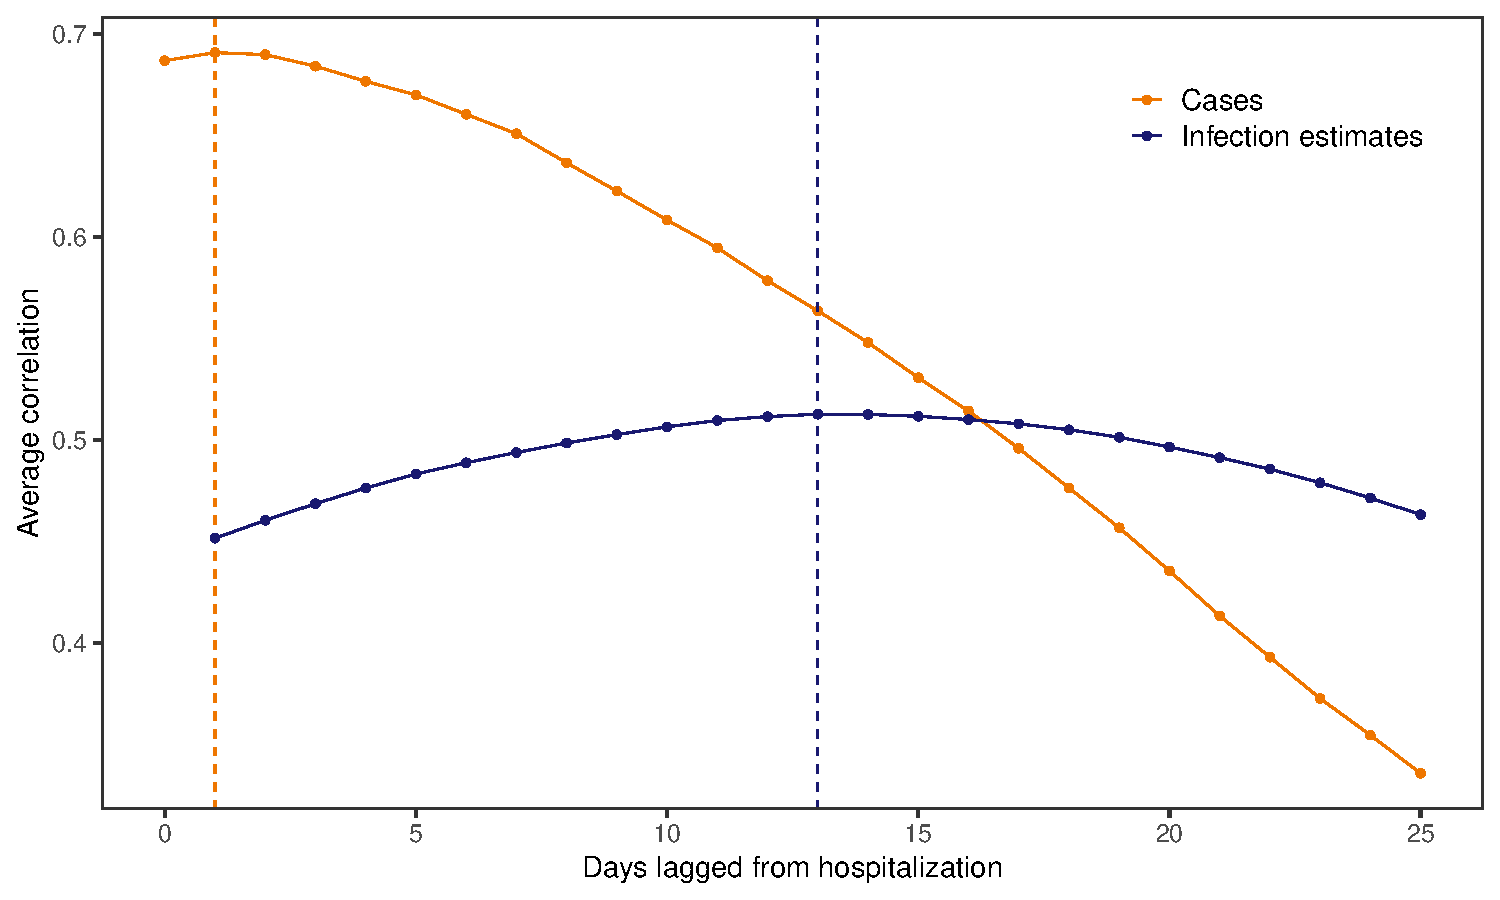
\includegraphics[width=.45\textwidth]{infect_case_hosp_lag_corr_F24.pdf} 
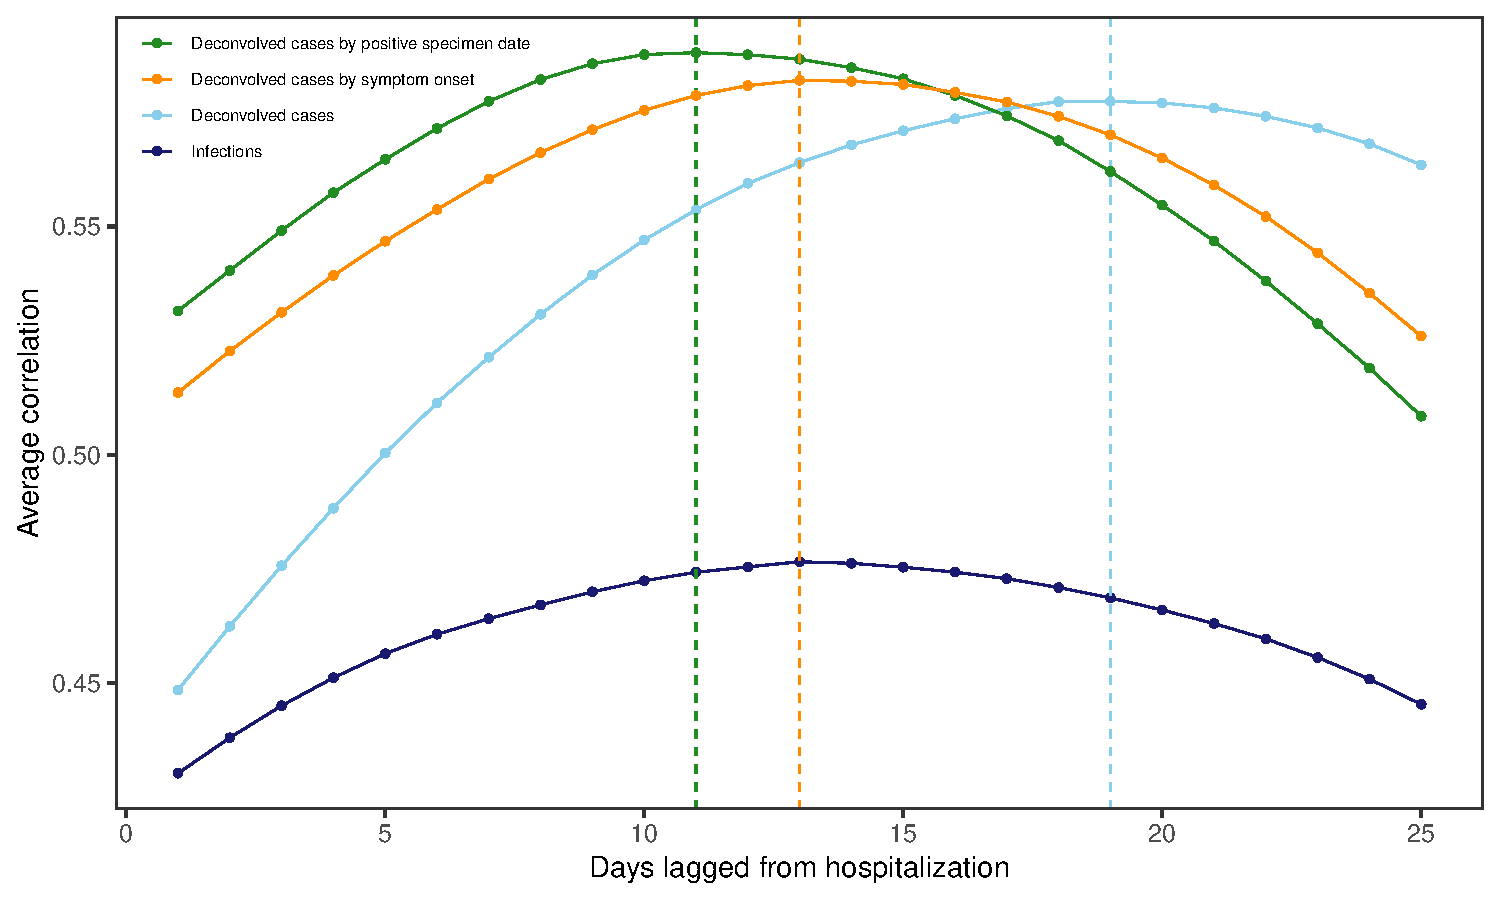
\includegraphics[width=.45\textwidth]{adj_unadj_pi_no_inc_hosp_lag_corr_F24.pdf} 
\caption{Spearman's correlation between the different case/infection ratesand
hospitalization rates per 100,000. These are calculated for each
lag, state and rolling window of 61 days before averaging. 
The vertical dashed lines indicate the lags
for which the highest average correlation is attained. \attn{Let's do one panel
with cases, deconvolved cases, and infections.}}
\label{fig:correlations}
\end{figure}
    

% In terms of the average correlation produced, the deconvolved case estimates by
% infection onset and the deconvolved case estimates by positive specimen date
% reach almost the same maximum average correlation. While that is not a clear
% differentiator by itself, there is a clear time-based benefit of opting for the
% infection estimates by the date of infection onset over symptom onset because
% they provide similar information on hospitalizations about 6 days before the
% latter tends to occur.

Unsurprisingly, the deconvolved case and infection estimates achieve their
maximum correlation at the same lag \attn{I don't think so...}. And yet, the average correlation to
hospitalizations tends to be greater for the deconvolved case estimates than for
the infection estimates. This finding may
stem from a difference in disease severity between the reported and unreported
infections: unreported infections tend to be less severe and less likely to
lead to hospitalization than those that are reported.




\subsection{Estimating infection-hospitalization ratios}
\label{sec:ihrs}

As a counterpart to the correlation analysis, we compute the time-varying
infection-hospitalization ratios (IHRs) for each state using the correlation
maximizing lag. We similarly compute the
case-hospitalization ratios (CHRs) using their correlation maximizing lag for
for comparison (\autoref{fig:IHR_7dav}). 

For each state, the CHRs tend to be larger and noiser relative to
IHRs. This supports our claim that the reported infections are more
likely to require hospitalization than the unreported infections. Both the IHRs
and CHRs exhibit similar geospatial and temporal trends as are noted for
infections. Namely, states that are close in proximity (such as Ohio,
Pennsylvania, and Virginia) tend to exhibit similar patterns in the IHRs and
CHRs over time. In addition, there are similar spikes observed across many
states during waves of infections that are driven by prominent new variants. For
example, many states exhibit a striking spike in hospitalizations in mid-2021,
which coincides with the rapid takeover of the Delta variant during that time
\citep{hodcroft2021covariants}. This finding aligns with previous studies that
found an increased risk in hospitalizations with Delta in comparison to other
variants \citep{twohig2022hospital, nyberg2022comparative}. Similarly, during
the fall of 2020 there tends to be another spike in the IHRs that rivals or
surpasses that observed during the time of Delta (which is the case for states
like New York or Wyoming). 

There does not tend to be a strict upward or downward trajectory or even a
mild waning pattern in the IHRs, as one might expect with later variants that are
more infectious but result in fewer hospitalization
\citep{lorenzo2022covid, blauer2022compare}. Overall, we observe intermittent
spikes that punctuate longer periods where the IHRs tend to stablize slightly below 0.2
hospitalizations per infection. These spikes tend to align with the emergence of
new variants. \attn{0.2 seems wrong. Is the IHR actually H/I? or are the units
not quite right (e.g., H/1M / I/100K)?}

While we computed and compared CHRs and IHRs for all states, it is important to
note that both likely to vary within states and depend on confounding variables
such as age and the presence of major comorbidities
\citep{russell2023comorbidities}. Therefore, it would be beneficial to account
for such variables in their calculations by, for example, stratifying infections
and hospitalizations by age to produce age-specific estimates of the IHRs for
each state~\citep{fox2023disproportionate}.



\begin{figure}[!tb]
\centering
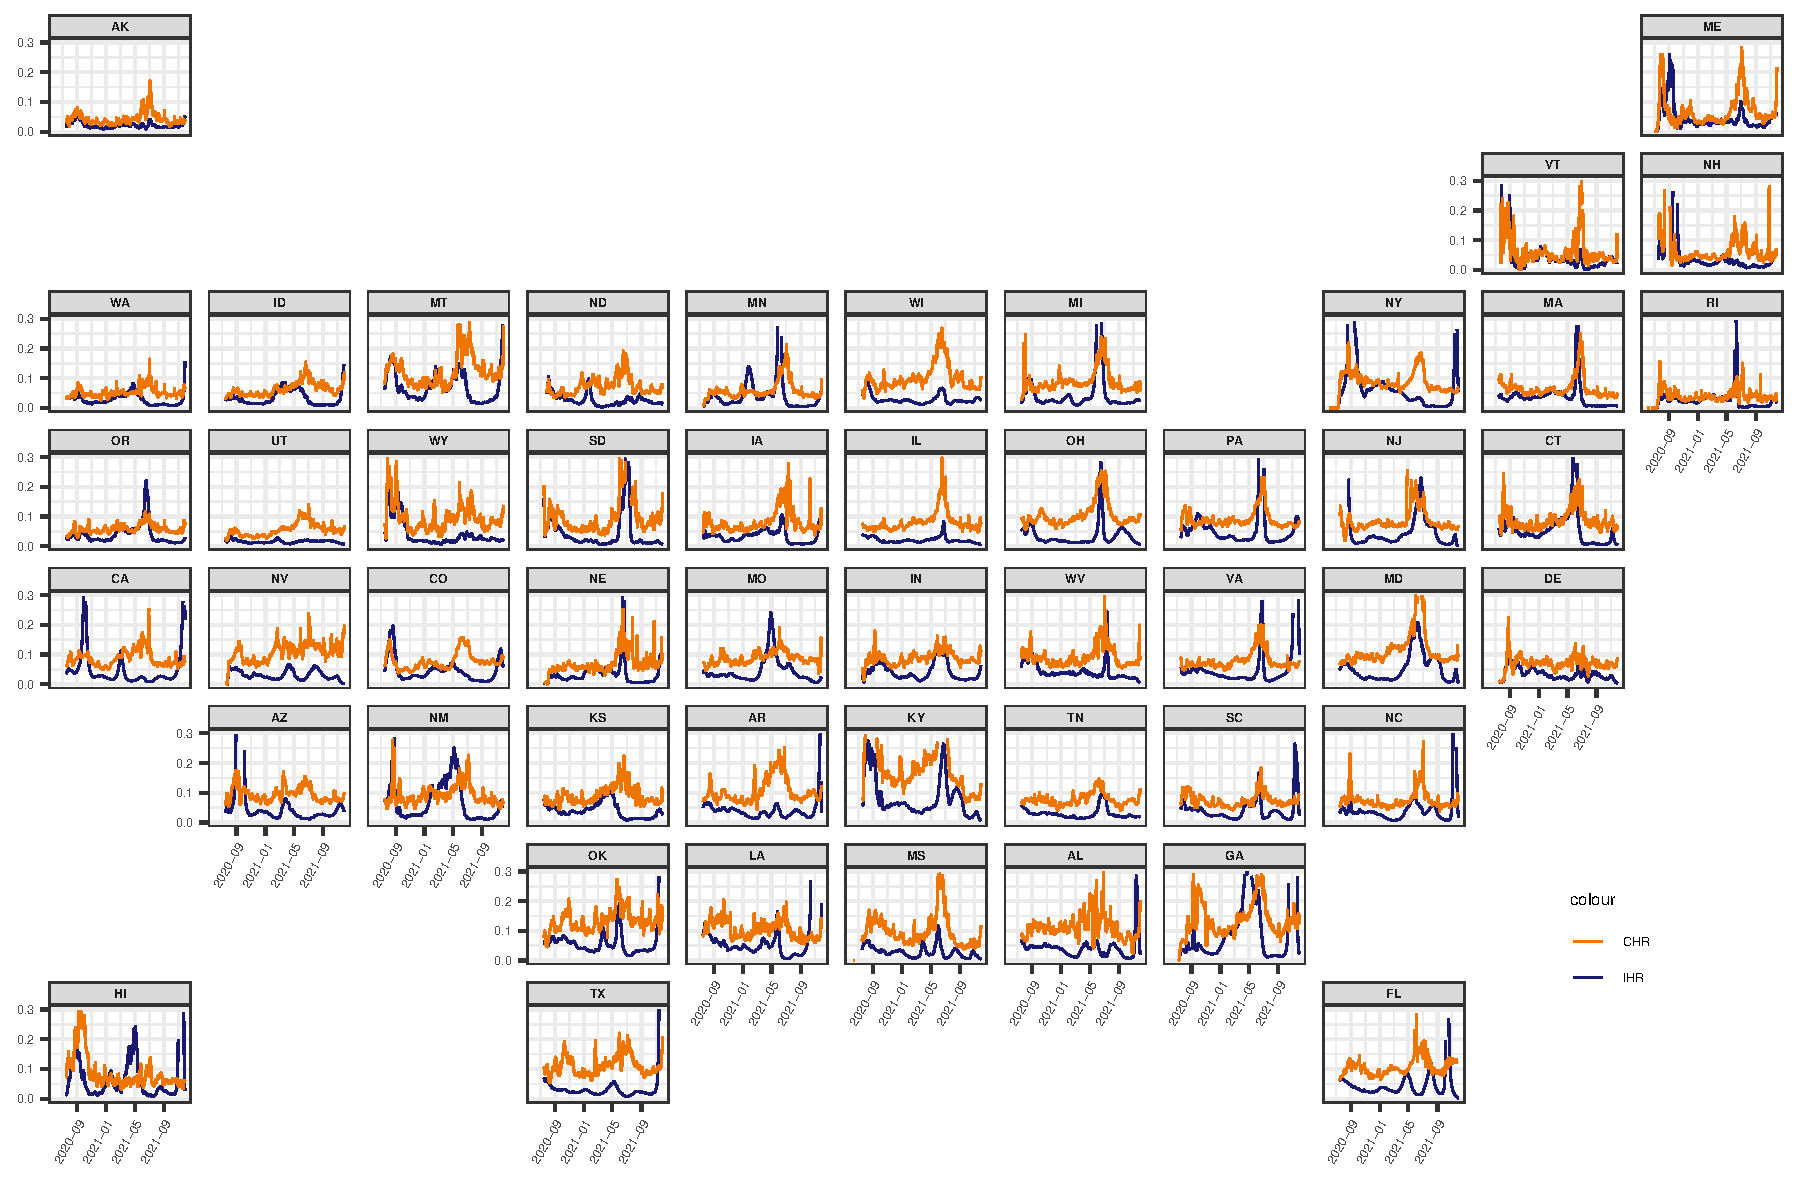
\includegraphics[width=.99\linewidth]{IHR_7dav_F24.pdf}
\caption{Time-varying IHR and CHR estimates for each state from June 1, 2020
to November 29, 2021, obtained using the corresponding optimal lag from the
systematic lag analysis. Note that the infection, case, and hospitalization
counts are subject to a center-aligned 7-day average to remove spurious day
of the week effects. Also note that the different starting points across
states are due to the availability of the hospitalization data.}
\label{fig:IHR_7dav}
\end{figure}


\subsection{Disease burden and viral transmission}

\attn{I'm not yet sure what to do with this. Some of it should go into one of 
the sections above.}

From reconstructing the time series of COVID-19 infections per $100,000$
population for each \US state from June 1, 2020 to November 29, 2021, we
observe rates of infections that vary in intensity and disease burden across
space and time (\autoref{fig:state_infect_est}, \autoref{fig:six-states}).  
Most states present at least two major spikes in infections - the first starts
in the fall of 2020 and extends into the winter season, while the second starts
in the late summer of 2021 and proceeds into the mid-fall. These represent major
waves driven by the Ancestral and Delta variants. Similar patterns in the major
surges of infections are observed in nearly all states, though to varying
degrees. In general, greater similarities in the strength and magnitude of
outbreaks are found to emerge in the clusters of states that border each other.

To avoid encroaching upon possible boundary issues with ending the estimation
during a time of volatility (the period of the Delta-Omicron transition), we
focus on the infection estimates prior to November 1, 2021. The largest observed
outbreaks prior to this time were observed in the late summer or early fall of
2021 in Georgia, Louisiana, Idaho, Montana, and Wyoming which suggests a similar
spread of the virus in small clusters of states that are in close geographic
proximity. During this time, the two states that have the attain the highest
rate of infections per 100,000 on single day are Georgia with about $451$
infections per 100,000 on August 15, 2021 (95\% confidence interval: $[334,
567]$) and Idaho with $451$ on September 7, 2021 (95\% confidence interval:
$[312, 590]$). These are closely followed by Montana with $432$ on September 8,
2021 (95\% confidence interval: $[282, 581]$), Louisiana with $431$ on July 20,
2021 (95\% confidence interval: $[252, 610]$), and Wyoming with $350$ on
November 13, 2020 (95\% confidence interval: $[256, 444]$).

Prior to the Delta wave, the state that has the highest rate of infections per
100,000 on single day is Louisiana with about 358 infections per 100,000 on July
3, 2021 (95\% confidence interval: $[177, 539]$), followed by Wyoming with 349
on November 13, 2020 (95\% confidence interval: $[407, 546]$), South Dakota with
342 infections per 100,000 on July 3, 2021 (95\% confidence interval:$[177,
539]$), and Illinois with 340 infections per 100,000 on July 3, 2021 (95\%
confidence interval: $[177, 539]$). During this time, 74\% of the top rates for
each state were observed in the late fall or winter of 2020.

The period of lowest viral transmission is observed in the summer and fall of
2020. During this time, the state of New Hampshire achieves the lowest weekly
rate of infections of 0.01 infections per 100,000 for the week of September 13,
2020. In the summer of 2020, Vermont maintains a rate under 10 infections per
100,000 from the week of June 1, 2020 to August 30, 2020, which is the longest
continuous stretch observed for any state.

From a brief inspection of the geo-contiguous states, we can observe similar
patterns in surges and periods of waning over time, suggesting that states who
share similarities in climate and topography performed similarly to each other.
More precisely, we can observe neighboring states such as New Hampshire and
Massachusetts or Idaho and Montana that present waves that mirror each other in
amplitude and timing. 

Interestingly, the two states that are geographically removed from the
contiguous United States, Alaska and Hawaii, tend to perform quite differently
from each other later in the pandemic. Alaska generally presents significantly
greater rates of infections than Hawaii especially during the Delta era. This
suggests that it is not so much the non-contiguity aspect as it is other
distinguishing factors that lead to lower infection rates.


%\subsection{Sensitivity analysis}
% This section is under construction
%The infection estimates exhibit modest changes under different assumptions about the
%variant-specific incubation periods, the construction of the delay distribution (the
%window size for the considered onset dates), the fraction of new infections over time, and
%the population estimates (see Supplementary Materials Section X). 
% Potentially compare ww a_t ratios over the time period as well (ie. do they fall in the confidence bands for a_t estimates
% from the ss model)?
% \attn {Add a sentence or two about what is meant by modest changes... Did any of these result in noticeably higher or lower (biased) estimates of infections? To what extent (ie. an additional X infections)? For what states?}
% Do these sensitivity analyses + update this link accordingly.
